% --------------------------------------------------
% Implementation
% --------------------------------------------------
\chapter{Implementation}

% Here you describe the detailed design of your solution and the details of the actual implementation. It may be appropriate to discuss aspects of design or implementation that were particularly problematic and/or novel. This section may well be one of the largest in your report and the exact contents will be unique to your project and so there are no general guidelines. Use of several sub-sections here is appropriate.

This chapter focuses on the overall implementation of the system and walks through how the several separate systems interface together and interact in a way that provides the user with a positive experience.

\section{Backend}

The backend of the system is implemented in Node.js and provides the API that the frontend will interact with through REST requests and WebSocket messages. TypeScript \cite{typescript} is being used rather than plain JavaScript in order to provide support for static types and catch more errors during the build time compilation rather than during run time.

\subsection{Database}

The database is a straightforward MongoDB \cite{mongo} implementation with two collections, one for exercises and one for activities. An exercise can have many activities but activities can only belong to one exercise.

%TODO: Relational mapping?

For the Node server to be able to make database calls the MongoDB API must be queried against, this is done by using the \textbf{mongoose} package \cite{mongoose}.

\subsection{REST API} \label{impl-rest}

To provide an API that a frontend can interact with to retrieve information from the database, a REST API is created with the Express framework \cite{express}. Creating an API endpoint with Express is a simple process that roughly follows the formula of:

\texttt{AppObject.RequestType("Endpoint", CallbackFunction)}

Where \textit{AppObject} is the variable representing the instance of the server. \textit{RequestType} is usually one of GET or POST. \textit{Endpoint} is a string representing the local path the handles the request and \textit{CallbackFunction} is the function that handles the request and sends the response.

so the code \texttt{app.get("/profile", callback)} is the function that would handle GET requests to the \textbf{/profile} endpoint. 

The only REST endpoints in the backend code are related to the exercises section of the system as those need to be stored in a global database. Most of the communication between the front and back is implemented through WebSocket connections.

\subsubsection{Get Exercise Endpoint}

The \textbf{/exercise} endpoint is a GET request that returns the related exercise in the database that corresponds with the ID that is sent along in the query string.

The callback function that deals with the request and sends a response is shown for this endpoint and it sends a response of 404 if it can't find the exercise based on the ID passed in the request and a 500 if there was an error with processing the request (such as if the database is down). Otherwise it will send a 200 and the exercise JSON object.

\begin{sexylisting}{/exercise endpoint}
server.get("/exercise", (req: Request, res: Response) => {
    const { id } = req.query;

    Exercise.findById(id)
        .populate("activities")
        .exec()
        .then(exercise => {
            if (exercise) {
                res.send(exercise);
                return;
            }
            res.sendStatus(404);
        })
        .catch(err => {
            res.status(500).json(err);
        });
});
\end{sexylisting}

\subsubsection{Create Exercise Endpoint}

The \textbf{/create} endpoint is a POST request used when a user makes a new exercise. Here the request object is broken down to get the parameters sent with the request and is turned into objects that can be inserted into the database.

The response is the endpoint that the frontend can use to navigate to the page for the newly generated exercise.

\begin{sexylisting}{/create endpoint}
server.post("/create", (req: Request, res: Response) => {
    /**
        Code to handle create request

        This is quite a lot of code refer to appendix %TODO:
    */
});
\end{sexylisting}

\subsection{Docker Integration} \label{impl-docker}

For the backend to have the ability to create and link Docker containers to a user running the application on the frontend it needs to be able to interact with the \textit{Docker Socket}. Every machine with an installation of the Docker Engine has a Docker Socket which is what the Docker CLI uses when commands are run against it.

There is a popular package on NPM called \textbf{Dockerode} \cite{dockerode} which enables interaction with the Docker API via whatever socket/path is provided in it's configuration.

The following code snippet shows the instantiation of the Dockerode package using the local Docker socket and exports it for use in other files in the project's backend.

\begin{sexylisting}{Create Docker instance and point it to local Socket}    
import Docker = require("dockerode");
const SOCKET_PATH = "/var/run/docker.sock";
const options = { socketPath: SOCKET_PATH };
export default new Docker(options);
\end{sexylisting}

\subsubsection{Provisioning a User Allocated Container} \label{impl-alloc}

Creating a container for every user that connects to the system requires the concept of a \textit{basic image}. This image is a Dockerfile which specifies the defaults for all user's environments. The Dockerfile is responsible for configuring the environment so that it is secure and pre-installed with all the tools that the user might need.

The basic image, comes with the following software pre-installed: \textbf{Alpine Linux Distro}, \textbf{Bash}, \textbf{Python3}, \textbf{Node.js}, \textbf{GCC} and \textbf{Git}.

Alpine Linux is the distribution that the base image of the container which is based on Ubuntu. Bash is a very common shell which is a better default than the standard \textit{ash} or \textit{sh} which are the shells that come with the Alpine image. Bash is important for the code execution aspect of the system which is explained further in \textit{Executing Code - \ref{imp-execode}}. Python, Node and GCC are chosen as those are the 3 runtimes that are supported by the system. Git is installed so if the user writes something that they want to be able to save they can use Git through the command line.

% TODO: Ref the dockerfile in the appendix
Some additional configuration that is done in this Dockerfile is the creation of the user account that users of the system will be operating as while they're connected to the container. By default the Docker engine sets the user of a container as root but this is obviously not appropriate for a system where anyone can play with a container so a low permission user is created called \textit{damien} who has their own home folder and ownership of that folder but everything under the root directory is protected.

The JavaScript to create the container for the user is a simple function call referencing the Docker API variable.

\begin{sexylisting}{Create container with options}
const container = await docker.createContainer({
    Image: "basic",
    AttachStdin: true,
    AttachStdout: true,
    AttachStderr: true,
    Tty: true,
    Cmd: ["/bin/bash"],
    OpenStdin: true,
    StdinOnce: false,
    name
});
\end{sexylisting}

This tells the API to create a container using the image with the label "basic" which is what the Dockerfile described above has the label of. The various \texttt{AttachX} properties tell the container if they should allow other processes to attach to this containers Standard Input/Output/Error which, as this container is emulated on the front end is required to be \texttt{true}. Tty refers to an old way of referring to the interface for a terminal. Without this option set to true it won't display in a way that looks like a traditional command line environment. Cmd is the command that the container should run once it's been created, in this case it needs to run bash. OpenStdin allows standard input to the TTY. StdinOnce will close the STDIN connection if an attached user disconnects, this needs to be off for this system as going between an exercise and a container will detach in the way that satisfies this requirement and it needs to be able to reconnect to the STDIN. The name property is simply the labelled name of the container which is displayed to the user when they connect.

\subsubsection{Provisioning an Exercise Container} \label{impl-exer-cont}

Provisioning the exercise container is more or less the same as the user's allocated container but it has to pause the allocated container so that resources aren't being wasted and then create the container for the exercise.

Exercise containers are created when a user enters an exercise and are destroyed when a user leaves the exercise. The are created the same way with the same configuration as the allocated containers however the image they are based from is the simplest REPL image that exists that relates to the runtime that the exercise is for.

\subsubsection{Executing Code} \label{imp-execode}

Getting code from the server to inside a file on the container and then executing is a fundamental requirement of this project and is achieved by taking advantage of Bash which is configured to come on every container created by the system.

The execute command in Docker (exec) is only capable of running a single command with arguments. In Bash however there is a way of chaining commands as arguments using the \textbf{-c} option. A JavaScript function called \texttt{getCodeSaveCommand} creates the command that the Docker execute command can run in order to save the file.

\begin{sexylisting}{Create command to save code to container}
export function getCodeSaveCommand(filename, code) {
    let cmd = ["/bin/bash", "-c"];

    code = code.replace(/`/g, "\\`");

    cmd.push(`echo "${code}" > ${filename}`);

    return cmd;
}
\end{sexylisting}

This snippet will add an escape character in front of all double quotes so that the double quotes don't finish the \texttt{bash -c} command and add command that saves the code to the specified file to the cmd array. This array is what the CMD option accepts. 

After the file has been saved successfully a message is sent to the client confirming the save and the client sends an attach request for the code execution so that the STDIN and STDOUT can be attached to the terminal emulator.

The execute command to run the code is more straight forward than the command to save it to a file.

\begin{sexylisting}{Creating the code execution command for the container}
export function getCodeExecutionCommand(filename, repl) {
    let cmd = ["/bin/bash", "-c"];
    
    if (repl === Repl.C) {
        return cmd.concat(
            `gcc ${filename} && ./a.out && rm a.out`
        );
    } else {
        return cmd.concat(
            `${repl} ${filename}`
        );
    }
}
\end{sexylisting}

This snippet works along the same lines as the previous however more steps are involved for the C compilation step as an output file is generated which has to be executed.

\subsection{WebSockets - Backend} \label{impl-ws-backend}

As mentioned in the Solution Approach (Section \ref{solapp-rtc}) the standard WebSocket client that is available as a browser API and on the backend a middleware package \texttt{express-ws} \cite{expressws} is being used to allow connections to the server using the WebSocket protocol.

\subsubsection{Endpoint Configuration} \label{impl-ws-config}

For the server to be able to create a WebSocket connection with clients and endpoint must be created that accepts the WebSocket protocol. 

\begin{sexylisting}{Setup of WebSocket Endpoint}
    server.ws("/", (ws: WebSocket) => {
        console.log("Connection Made");
        startBasicContainer(ws)
        {...}
    }
\end{sexylisting}

The snippet above shows that a WebSocket connection can be made to the root endpoint of the server and once the connection is made it is logged to the console and the function to create the basic user allocated container is called.

\subsubsection{Message Structure} \label{impl-ws-msg-struct}

WebSockets are only capable of sending strings of text in their messages however, as JSON is a way of representing objects through strings a template message guide can be created.

\begin{sexylisting}[label={code:ws-msg}]{WS message}
    const message = {
        type: MessageTypes.CONTAINER_STOP,
        data: { id }
    };

    socket.send(JSON.stringify(message));
\end{sexylisting}

This snippet shows that an example message which is a JSON object with two properties \texttt{type}, which represents the type of the message being sent, and \texttt{data} which is an object itself which contains any relevant information that might be useful for the other end of the socket. In this case the type of the message is a flag to stop a running container and the data is the ID of the container. This is sent after being stringify-ed by the built in JSON object.

\subsubsection{Message Types} \label{impl-ws-msg-type}

As can be seen above each message has a type. These types are processed through a \texttt{switch statement} which inspects the type, extracts the parameters from the \texttt{data} property and makes a function call.

\begin{sexylisting}{How the messages are processed by the backend}
    const { type, data } = JSON.parse(msg);
    switch (type) {
        case "Container.Pause":
            // Used when focus is lost from tab
            console.log("Pausing container");
            stopContainer(ws, data.id);
            break;
        case "Container.Resume":
            // Used when focus is resumed via tab
            console.log("Resuming container");
            resumeContainer(ws, data.id);
            break;
        {...}
\end{sexylisting}

The first thing that is done when the message is received is, as the message is a string, it is parsed into JavaScript objects and the \texttt{type} and \texttt{data} properties are extracted. The \texttt{type} is switched against and based on what the value of it is. A string is logged to the console showing what action the server is performing and a function is called which will always pass the WebSocket object (so the server can reply) and then passes any relevant data that is required by that function. 

\subsubsection{WebSocket Streams} \label{impl-ws-streams}

Streams is a concept in programming which quite directly means a \textit{stream of data}. Streams are used most often to act on a huge amount of data in a more performance focused way. Streams of events are the types of streams that are used in this project however as the Docker containers are able to stream their STDIN and STDOUT. Using the Node.js Stream API it is possible to \texttt{pipe()} these streams over WebSockets.

The package \texttt{websocket-stream} is used in the server to enable the streams to be piped over the WebSocket connection.

\begin{sexylisting}{Endpoint which connects the container stream to the WebSocket}
server.ws("/connect", (ws: WebSocket, req: Request) => {
    const stream = websocketStream(ws, { binary: true });
    console.log("Trying to connect streams");

    attachSocketToContainer(
        stream,
        req.query.id,
        req.query.bidirectional,
        req.query.logs
    );
});
\end{sexylisting}

This snippet shows that a WebSocket connection can be opened to the \texttt{/connect} endpoint of the server where a stream will be created from the WebSocket. When the connection is made a function is called to attach the WebSocket stream to the container stream and it passes the stream created by the websocket-stream package, the id of the container to attach the stream to, whether the stream is bidirectional (allows STDIN and STDOUT) and if the previous logs from the container should be allowed.

Streams are a core concept in Node.js so passing one stream to another is simple.

\begin{sexylisting}{Attachment of the container stream to the WebSocket stream}
container.attach(
    {
        stream: true,
        stdout: true,
        stderr: true,
        stdin: isBidirectional,
        logs: showLogs
    },
    function(err: Error, stream) {
        {Error Handling here...}
        console.log("Stream Connection Established!");
        if (isBidirectional) {
            stream.pipe(wss);
            wss.pipe(stream);
        } else {
            stream.pipe(wss);
        }
    }
);
\end{sexylisting}

The snippet above is showing the Docker API making a call to attach to the running container which was calculated based off the ID passed to the function. The options show that the \texttt{stream} option is set to true, the \texttt{stdin} option is dependent on if the stream is set to be bidirectional or not and the \texttt{logs} are also determined by the parameter passed from the query string.

The callback function does error handling and then will pipe the container stream to the WebSocket stream. If bidirectional flow is enabled, it will also pipe the WebSocket stream to the container. 




\section{Frontend}

The general approach for developing the frontend of the project is stated in Chapter \ref{solapp} in Section \ref{solapp-frontend} but a number of other packages were used to make the development of the solution smoother and less error prone. Namely, TypeScript \cite{typescript} was used rather than plain JavaScript and Styled Components \cite{styledcomp} was used in addition to regular CSS to make implementing the design more straightforward.

The frontend consists of 4 pages or screens all of which have varying degrees of functionality and interaction with both the backend and the user.

\subsection{WebSockets - Frontend} \label{impl-ws-frontend}

The WebSocket configuration is fairly similar to the backend. The browser has the WebSocket object in it's global scope so there is no need to import a package like had to be done for the backend.

All the configuration for setting up the WebSocket connection and handling events is done in the \texttt{componentDidMount()} lifecycle of the entire application.

\subsubsection{Starting the Connection} \label{impl-ws-fconnect}

\begin{sexylisting}{WS connection setup}
    componentDidMount() {
        this.socket = new WebSocket('ws://localhost:4000/');

        this.socket.onopen = () => {
            console.log('Socket Opened');
        };

        {...}
    }
\end{sexylisting}

This snippet is creating a new WebSocket object and passing the URL of the path that the connection will be between. In this case it's the root WebSocket path that is shown in \ref{impl-ws-config} which initiates the container for the user.

\subsubsection{Receiving Messages} \label{impl-ws-fmsgrcv}

As the structure of messages is predictable (see \ref{impl-ws-msg-struct}) the same approach to deal with messages is used on the client-side as the server-side.

\begin{sexylisting}{WebSocket event listener}
    {...}
    this.socket.onmessage = (event) => {
        const { type, data } = JSON.parse(event.data);

        switch (type) {
            case MessageTypes.CONTAINER_START:
                console.log('Container Started');
                {...}
        {...}
    {...}
\end{sexylisting}

Here the WebSocket is registering an \texttt{Event Listener} which performs the same basic \texttt{switch statement} that the backend is performing.

After a message comes through, depending on it's content it will modify the global state of the application so that all screens are able to inspect the current state of the socket and any response that might be relevant to the functionality of that particular page. This global state is created with the built in Context API from React.

\subsubsection{Sending Messages} \label{impl-ws-fmsgsnd}

Sending messages is performed the exact same way as it is from the backend, shown in Snippet \ref{code:ws-msg}

\pagebreak

\subsection{Home Page} \label{impl-home-page}

The home page of the web app has the goal of showing users all the functionality of the system.

\begin{figure}[h!]
    \centering
    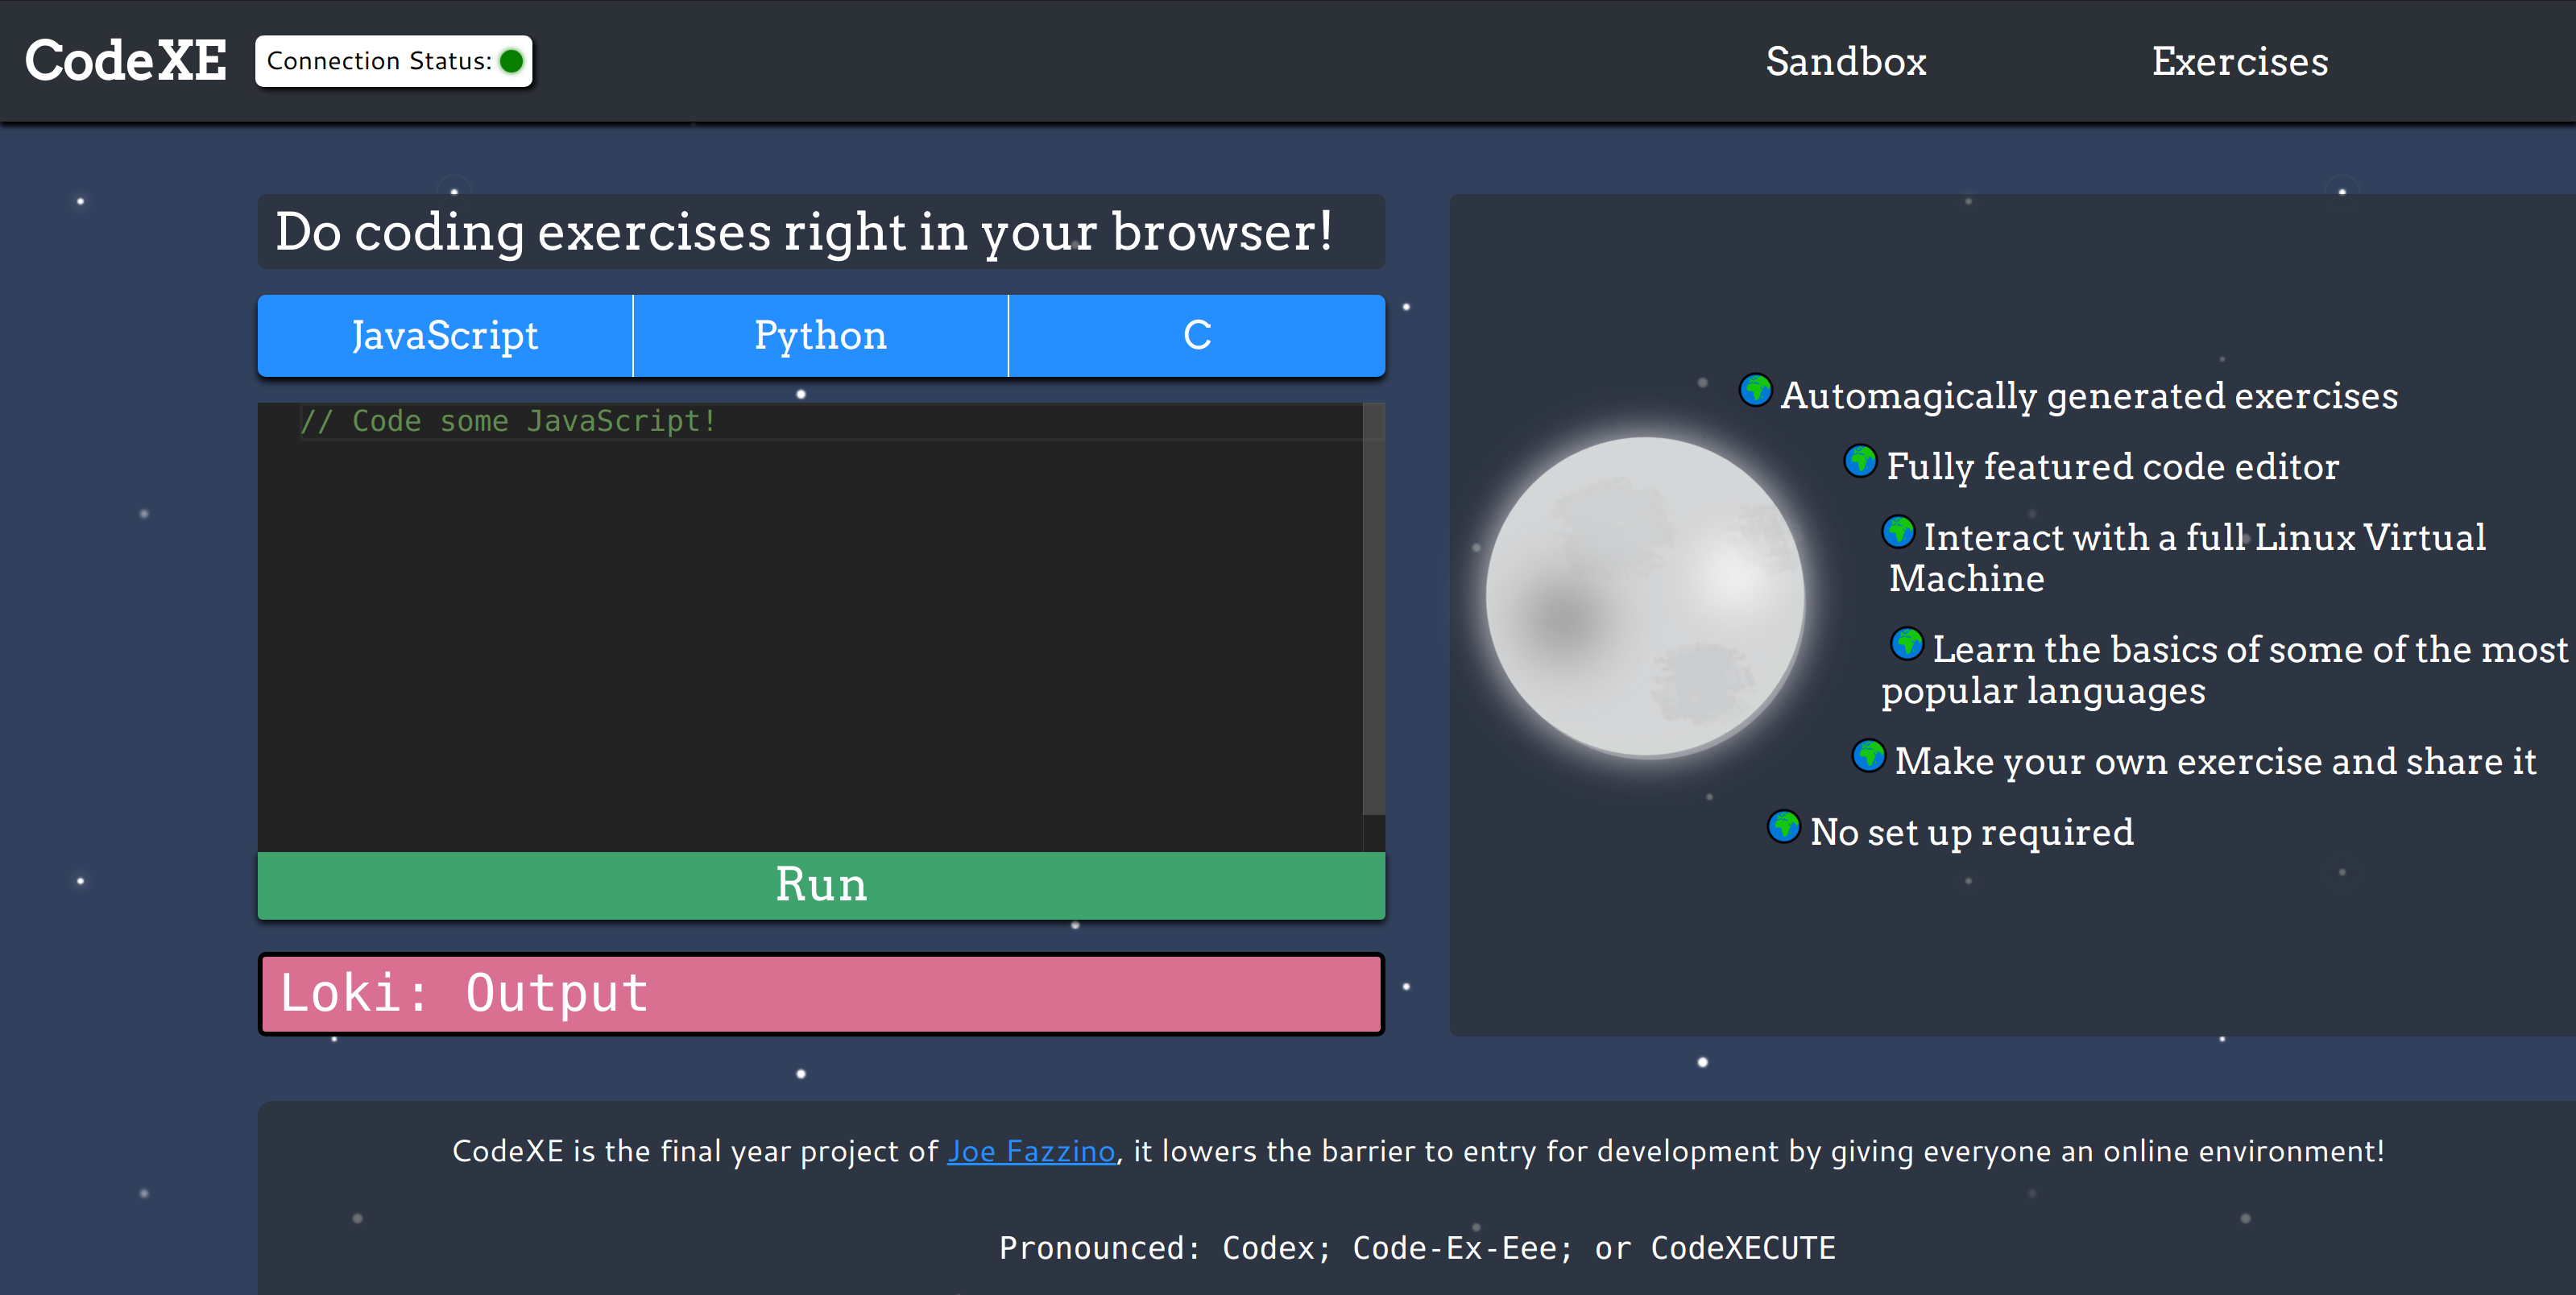
\includegraphics[width=\linewidth]{res/home_page.png}
    \caption{Landing Page/Home Page}
    \label{fig:homepage}
\end{figure}

At the top of the page there is a standard navigation bar which provides access to the homepage (by clicking on the name of the website), the sandbox page and the exercises page. The connection status uses a traffic light style green, yellow and red system to show the connection status to the users container. Clicking on it reveals the name of the container if connected and if there's an issue it says there's a problem.

\begin{figure}[h!]
    \centering
    
\includegraphics[width=\linewidth]{res/connection_status_with_popout.png}
    \caption{Connection status with container name}
    \label{fig:connection-popout}
\end{figure}

The home page also includes the Monaco code editor and a toggle for selecting a language so the whole functionality of the site can be sampled on this page. Picking any of the languages switches to the corresponding language and pressing \textit{Run} will execute the code and display the response in the pink output box below it which also displays the name of the container.

\subsection{Sandbox Page} \label{impl-sandbox-page}

\begin{figure}[h!]
    \centering
    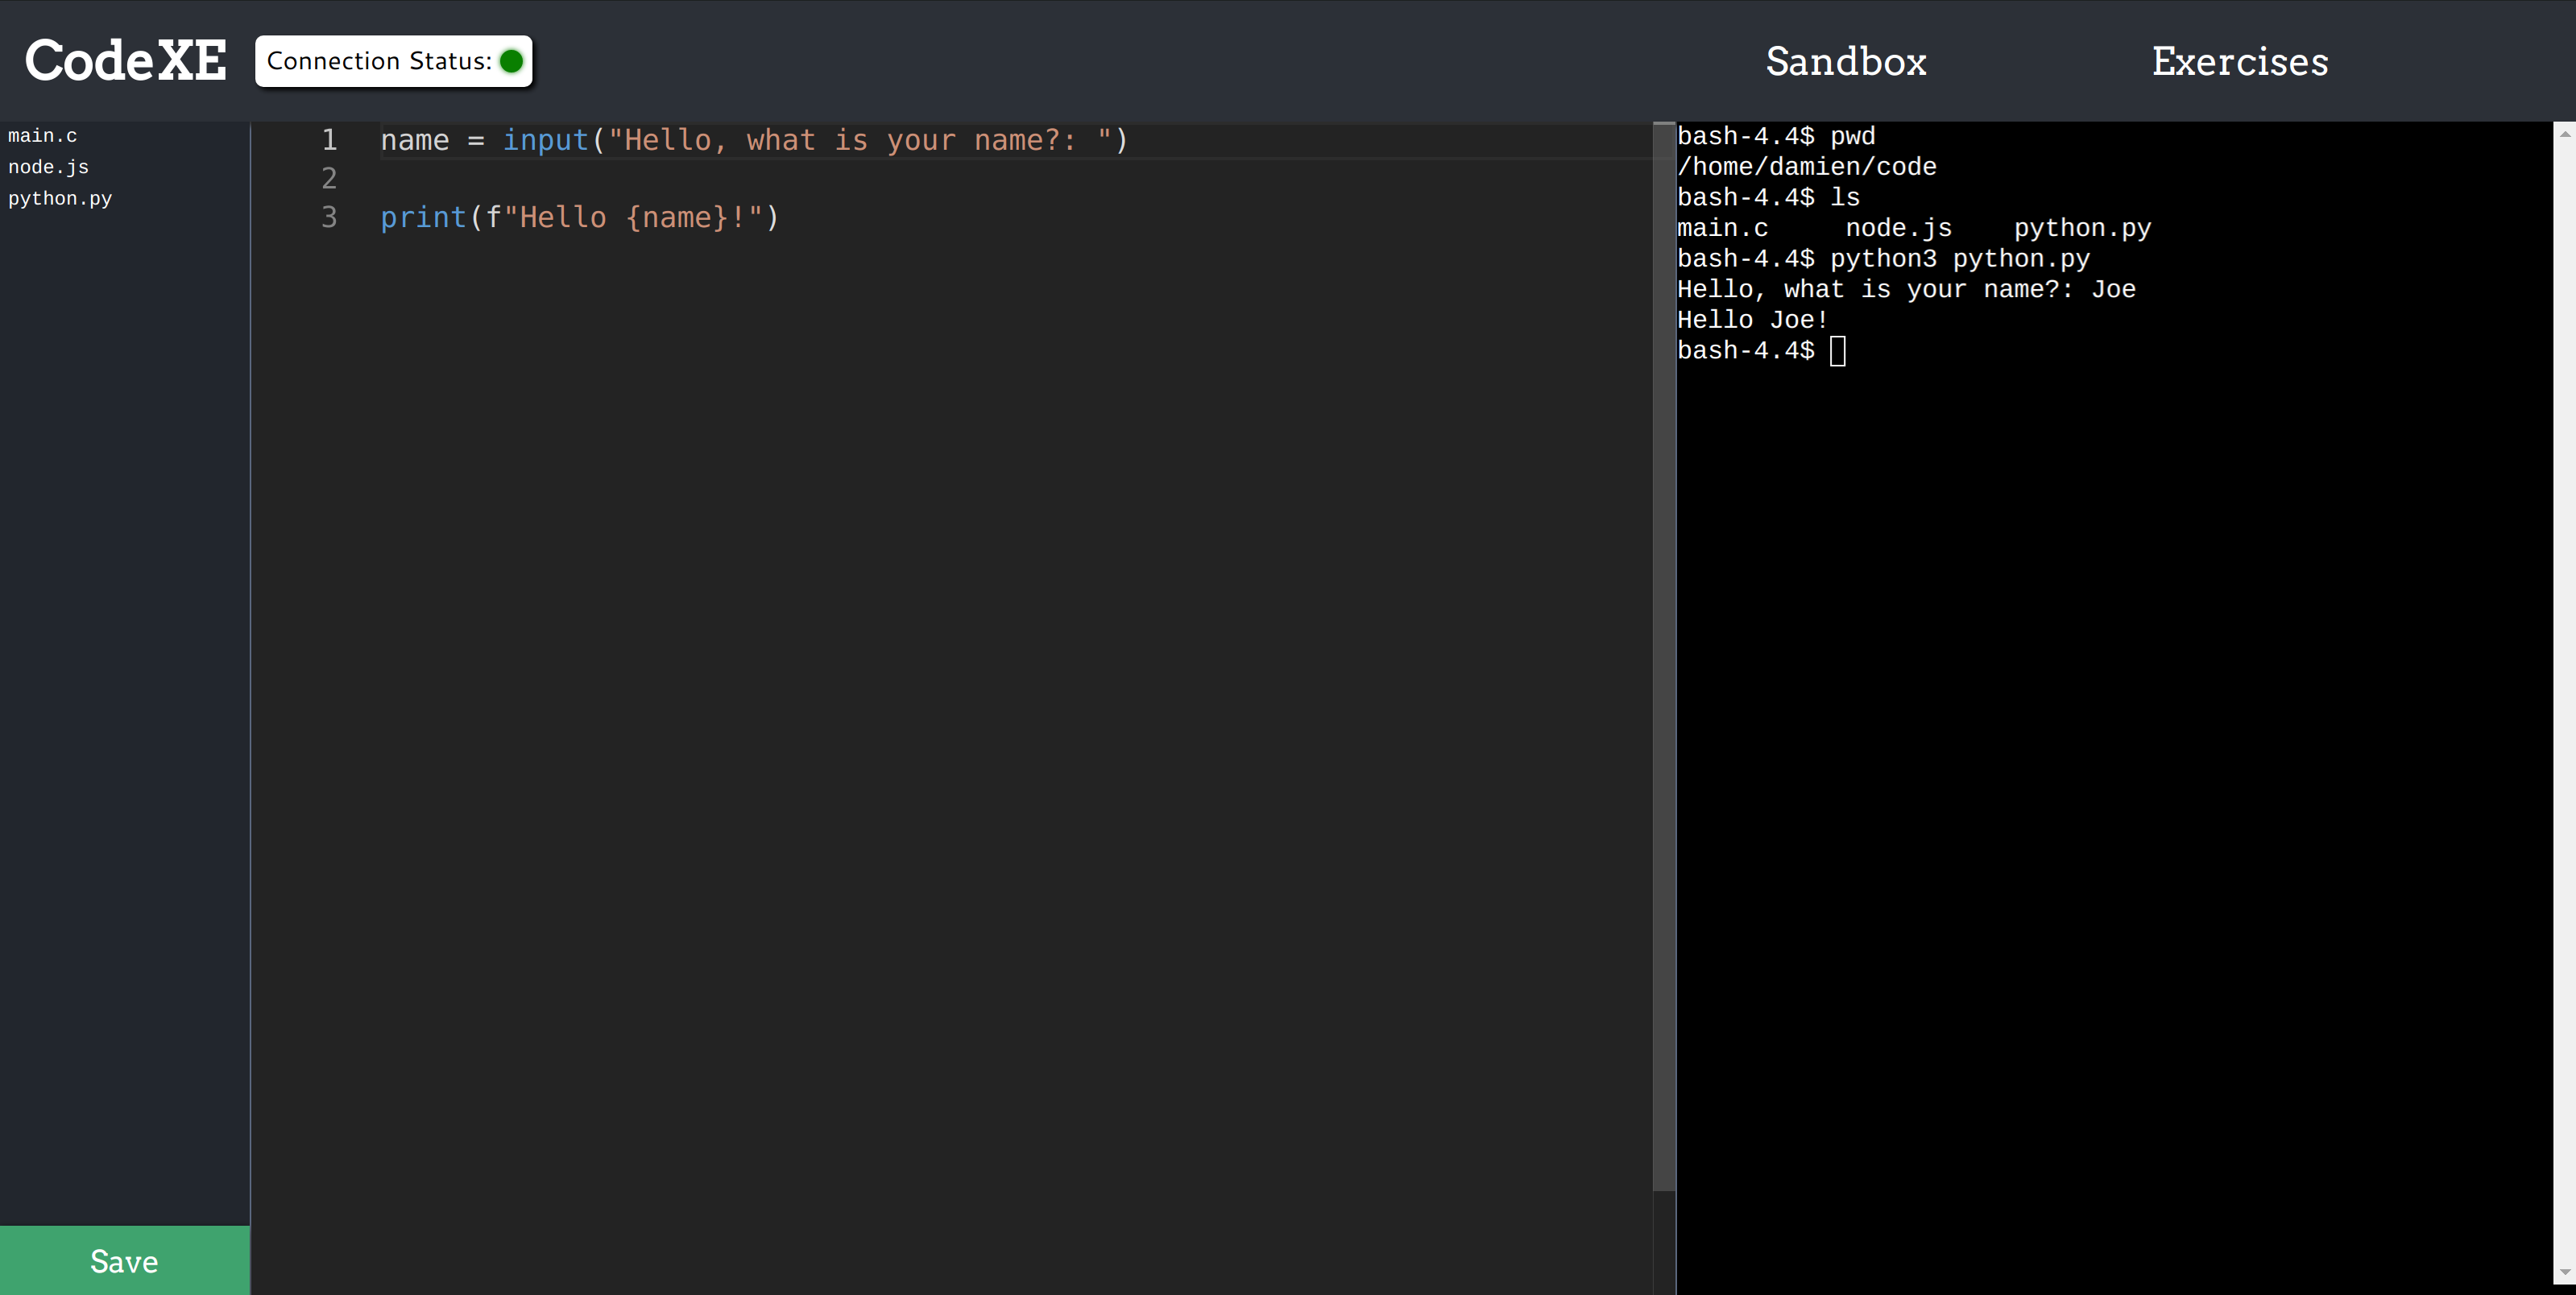
\includegraphics[width=\linewidth]{res/sandbox_page.png}
    \caption{Sandbox Page}
    \label{fig:sandboxpage}
\end{figure}

The sandbox page of the application has a simple file browser on the left which is created by passing the result of an \texttt{ls} Bash call on the container and sending the result to the client. In the middle is the Monaco code editor and on the right is the Xterm.js terminal emulator connected to the container's stream (see \ref{impl-ws-streams}). All three panes are resizeable.

The \texttt{Save} button will save the code to the container file that is currently open for it to be executed in the terminal emulator.


\subsection{Exercises Page} \label{impl-exercises-page}

\begin{figure}[h!]
    \centering
    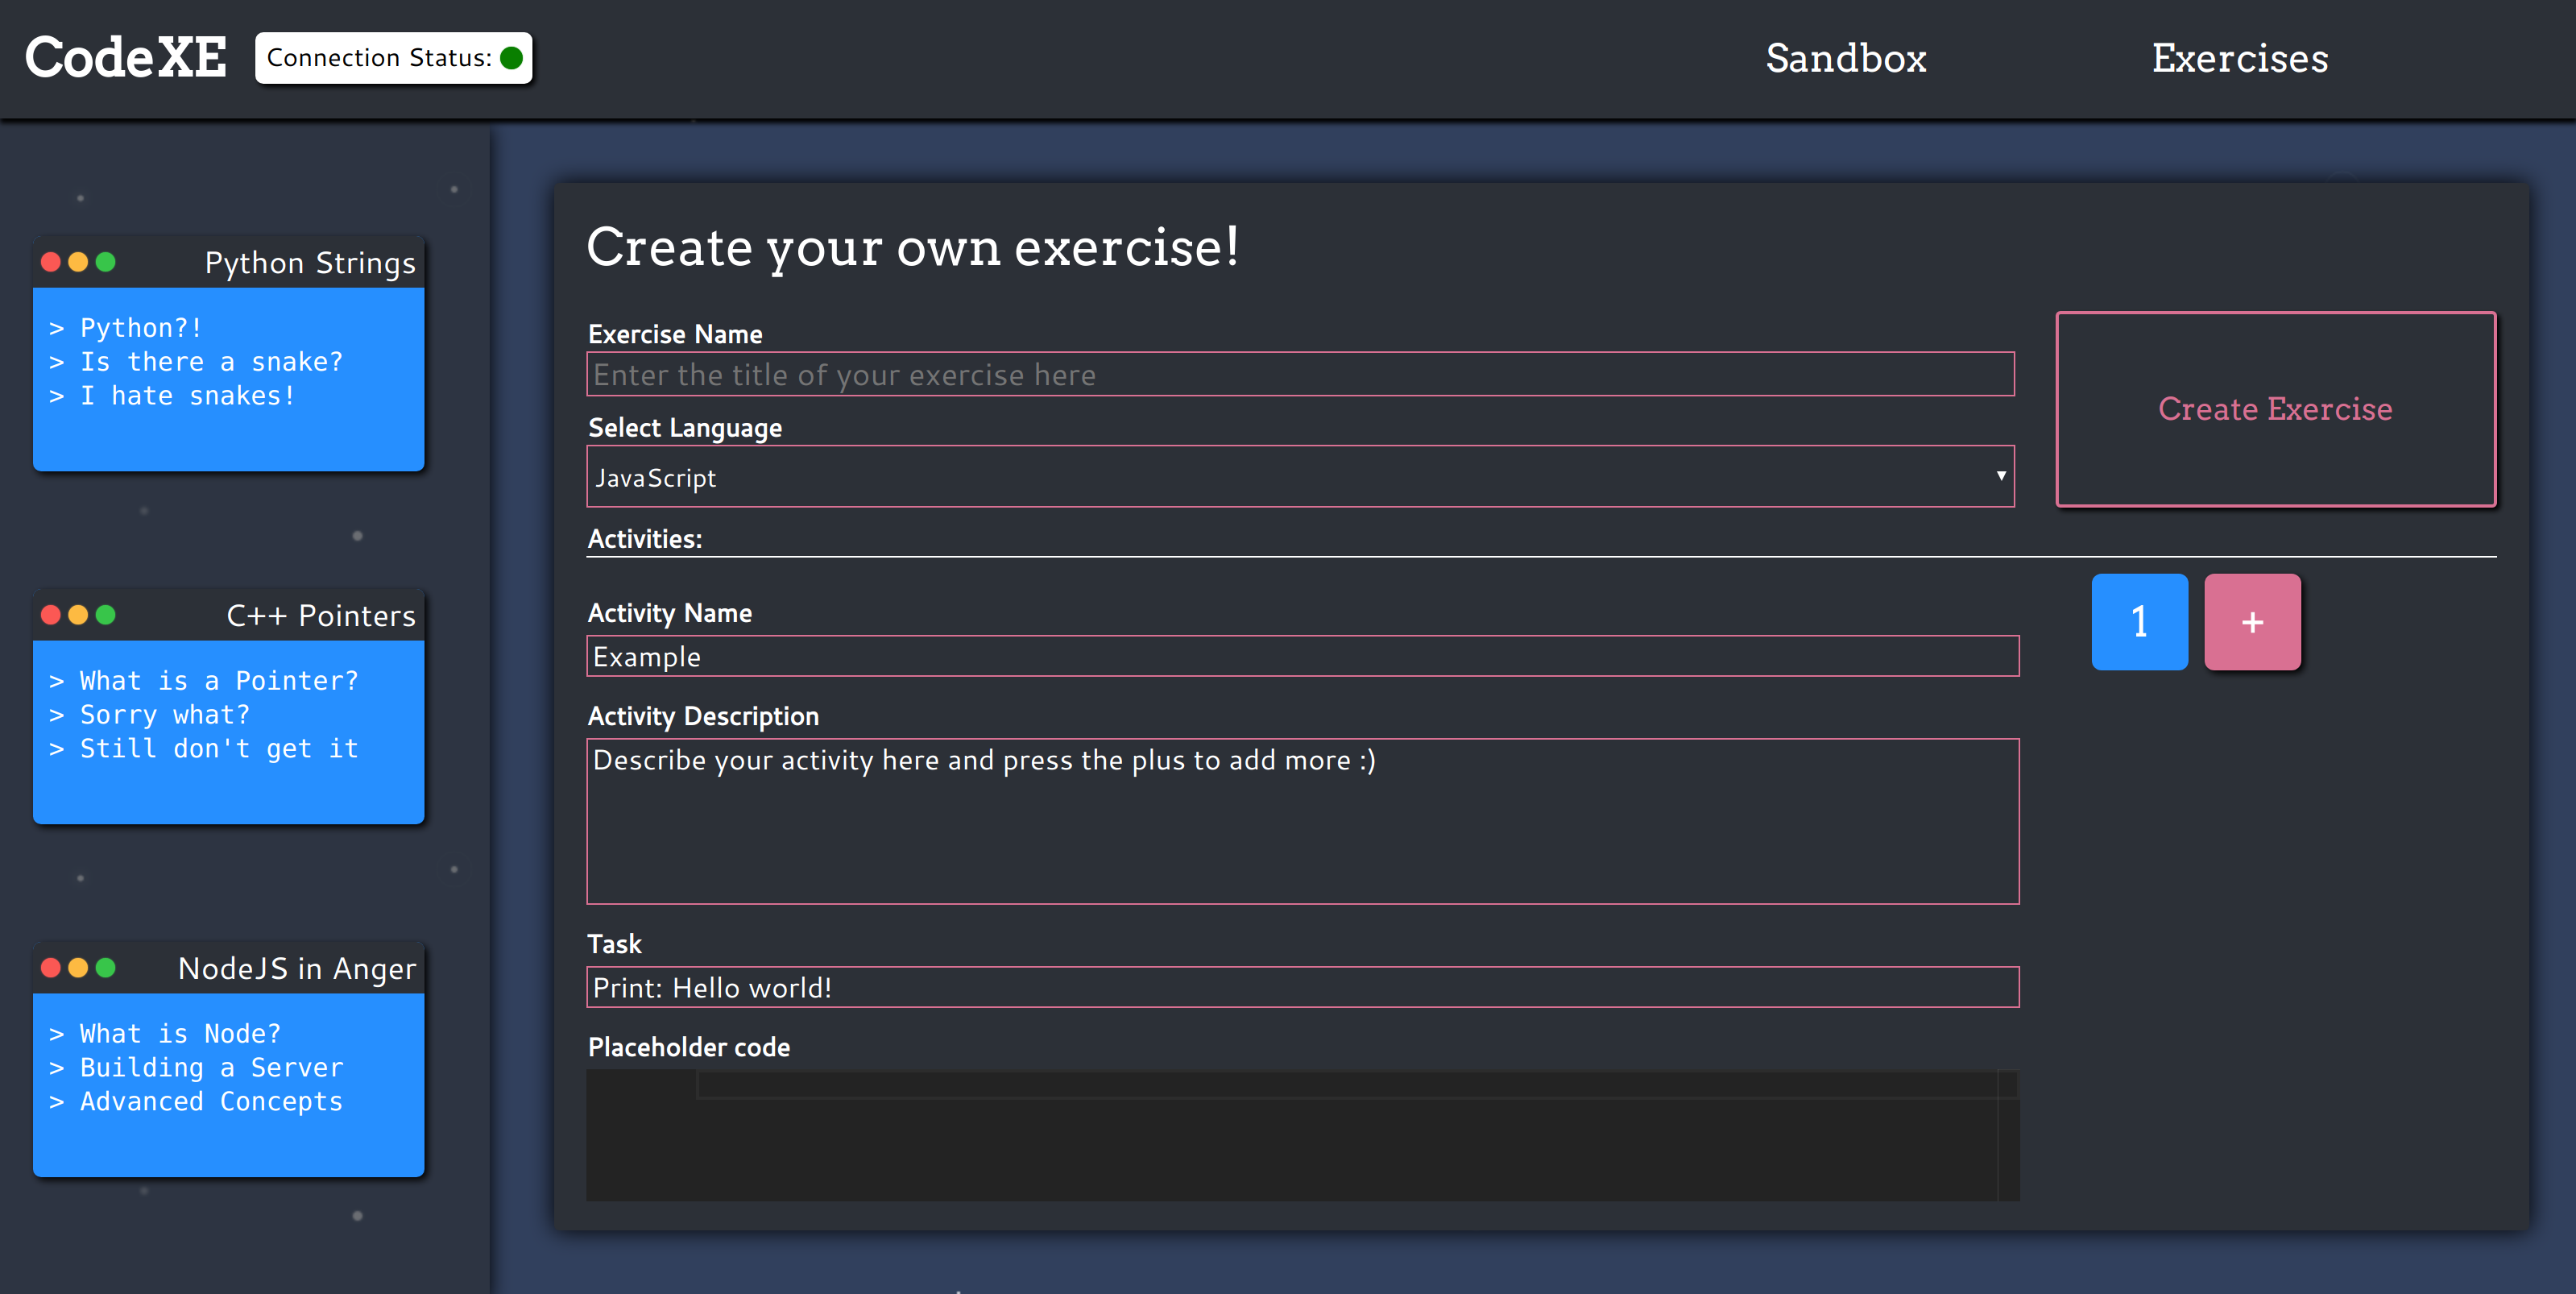
\includegraphics[width=\linewidth]{res/exercises_page.png}
    \caption{Exercises Page}
    \label{fig:exercisespage}
\end{figure}

The exercises page has a selection of available exercises on the left that will open the corresponding exercise screen. It also contains a form which users can create their own exercise in order to share with others or help mentor someone new to coding. Up to 15 separate activities can be made for any exercise.

\subsection{Exercise Page} \label{impl-exercise-page}

\begin{figure}[h!]
\centering
    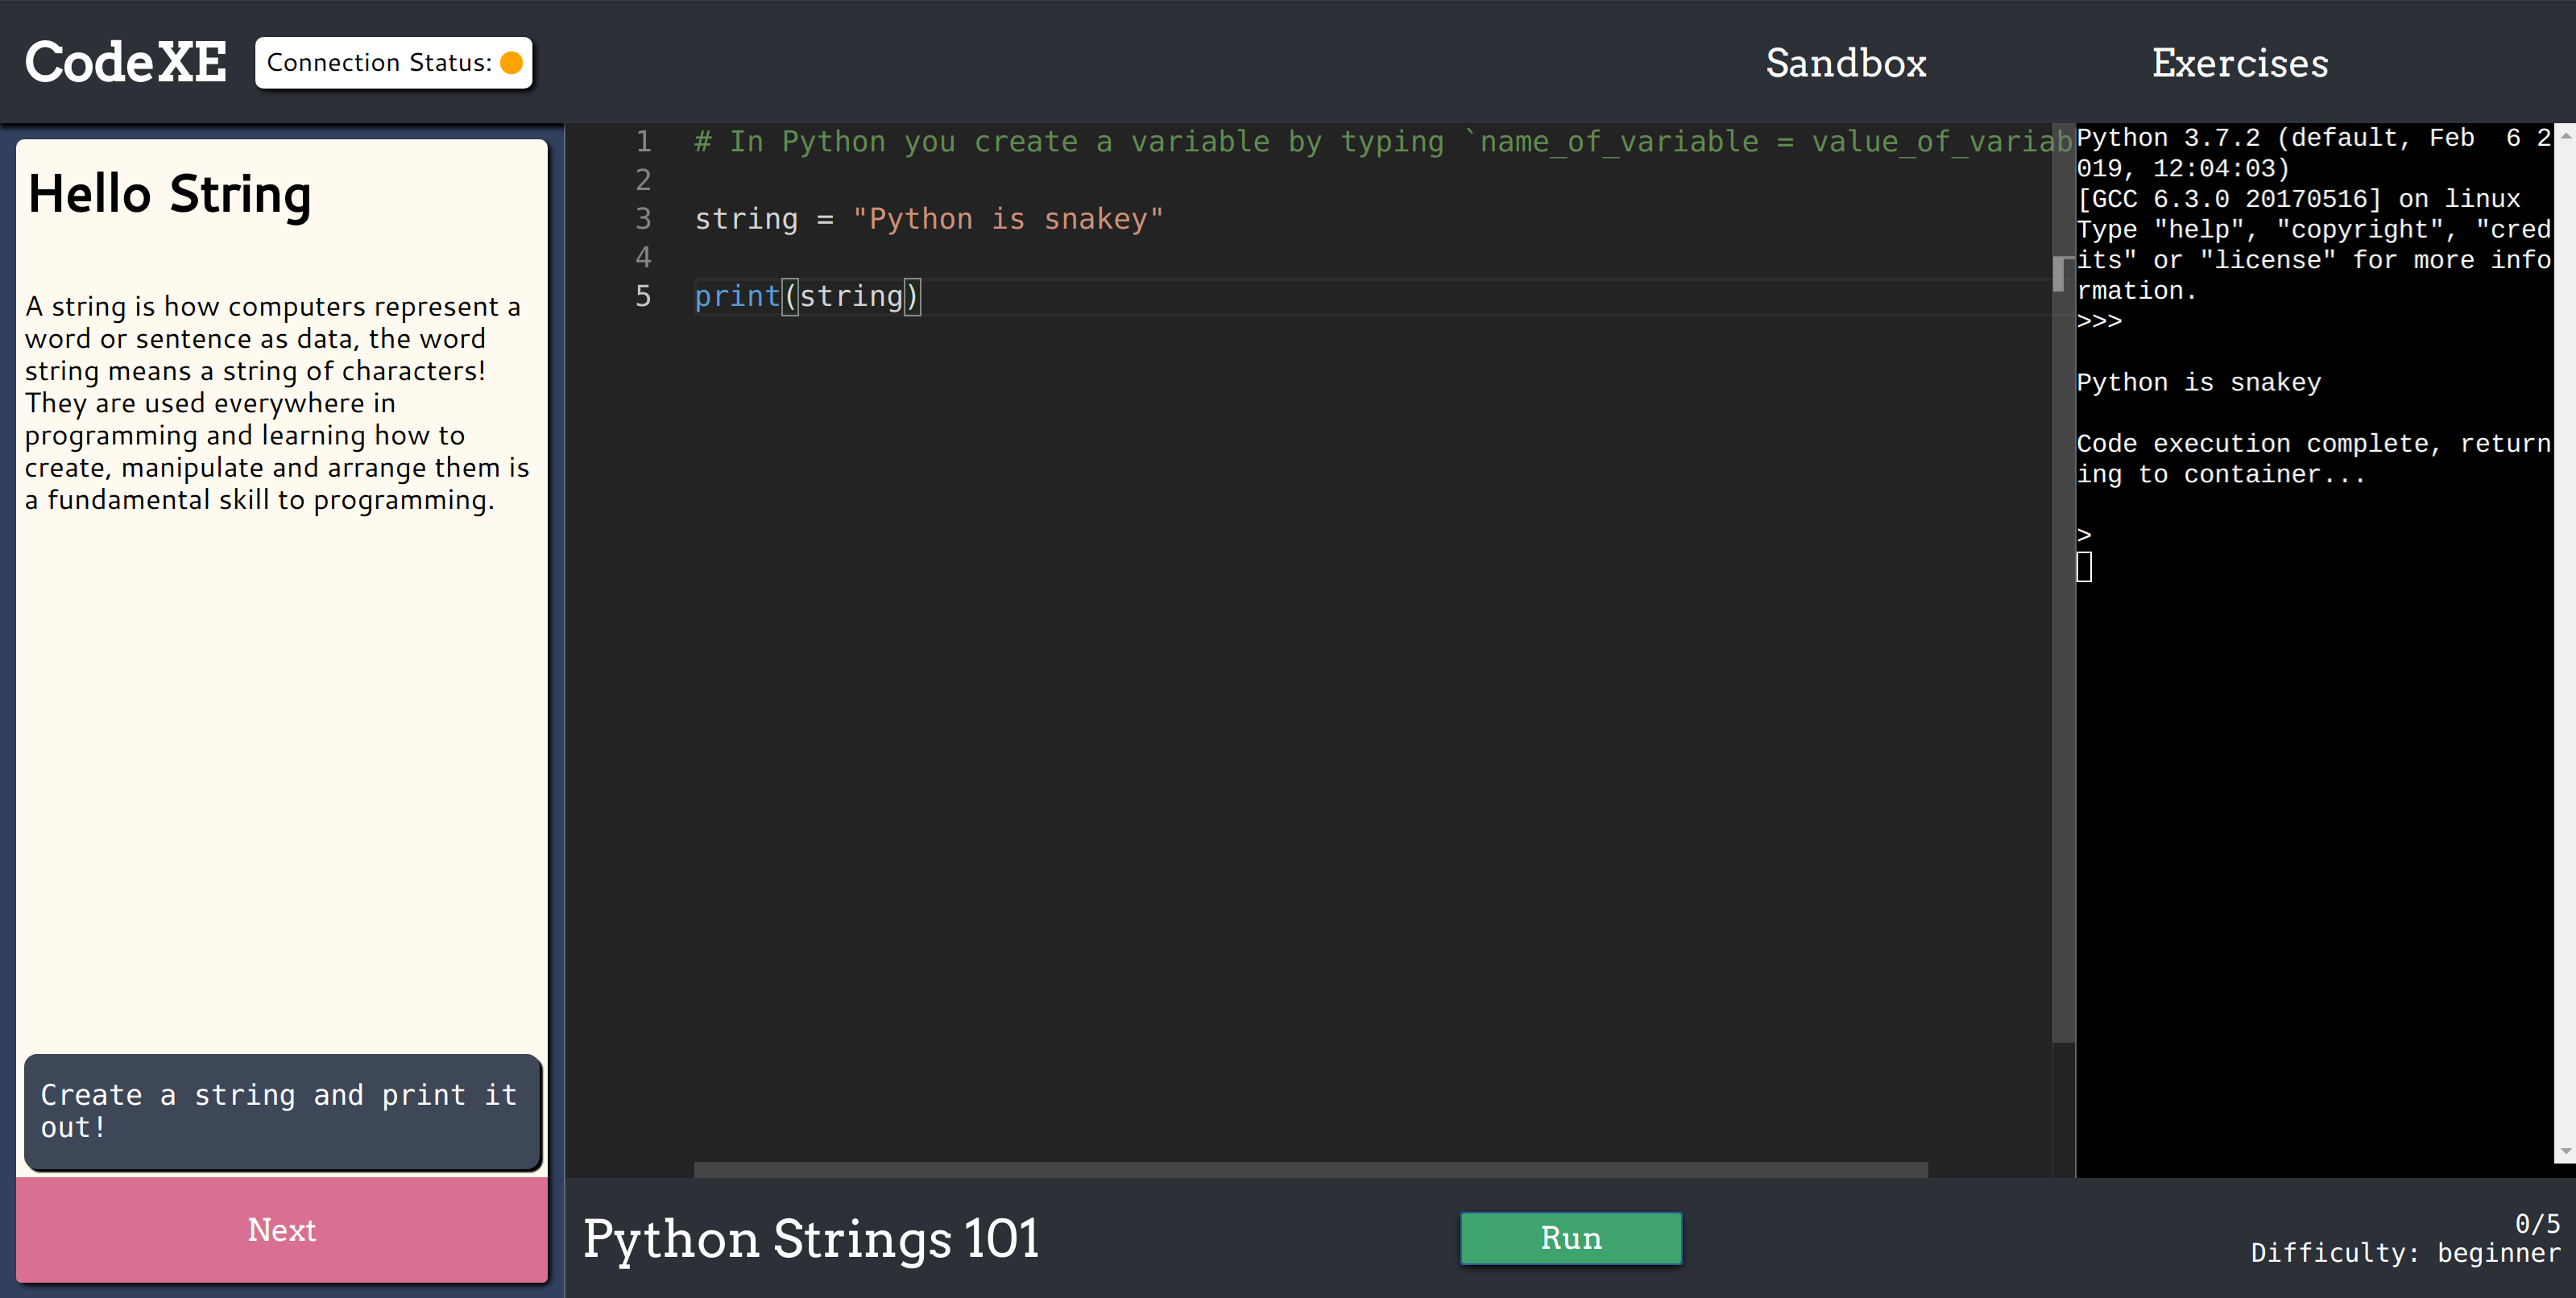
\includegraphics[width=\linewidth]{res/exercise_page.png}
    \caption{Exercise Page}
    \label{fig:exercisepage}
\end{figure}

The exercise page is what the user is greeted with when they interact with one of the exercises on the left of the exercises page. It displays the information for the user on the left of the specific activity they're on which is indicated by the counter in the bottom right. 

This page is the most complicated of all of user facing side of the application. When the \texttt{Run} button is pressed, the best user experience is to display the result in the terminal emulator. However, this is already attached to the exercise container and having more than once connection is not a viable solution. When \texttt{Run} is pressed the message to save the code must first be sent, when that comes back as successful, it detaches the terminal from the container and makes a new request to the \texttt{/connect} endpoint of the server (see \ref{impl-ws-streams}) to create but this time instead of passing the ID of the user's container it passes the ID of the exercise container.

When this execution finishes, the connection is re-established with the normal REPL attached stream to provide a seamless experience between playing with the REPL and executing code.

The \textit{Connection Status} in the nav bar has changed to a yellow status, this is due to the user's main container being paused while they are interacting with an exercise container. When the user navigates away from this exercise their main container is resumed and the exercise container is destroyed. 

\section{ContainMENT - Container Management} \label{impl-containment}

Although containers are light weight and not very resource intensive, creating containers on demand as users make a connection with the site will lead a fairly significant scaling issue if there is no management of them in place.

Currently there is only one ContainMENT tool in place which is \textbf{Ahab} (see \ref{impl-ahab}) but plans for additional tools are stated in Chapter \ref{conclusion}.

\subsection{Ahab} \label{impl-ahab}

Ahab is a Python script that is responsible for making sure that any containers that have been idle for too long or exited recently are removed after a reasonable length of time so that the resources allocated to those containers can be freed for other users. The script is designed to be run every five minutes automatically as a \textbf{Cron job}

\begin{figure}[h!]
    \centering
    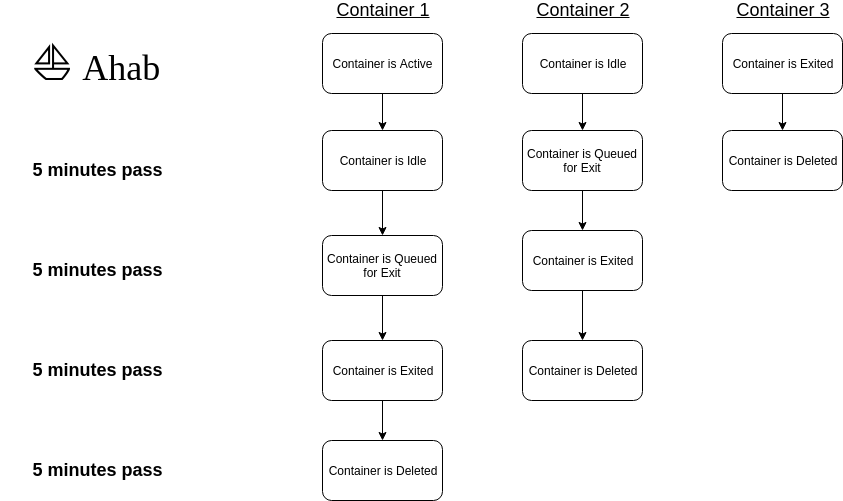
\includegraphics[width=\linewidth]{res/Ahab.png}
    \caption{Affect of script after every execution on containers}
    \label{fig:ahab-diagram}
\end{figure}

\pagebreak
